\section{Results}
\label{sec:results}

\subsection{Real-data benchmark}
\label{sec:experiments-real}

\Cref{tab:method-main-comparison} reports the main real-data comparison.
Classification uses the 21 datasets with results for every method; the full
classification collection has 23 datasets, and \nolinkurl{gisette} and
\nolinkurl{isolet} enter only the comparisons whose methods completed there
(\cref{app:methods}). Regression uses all 8 datasets. Within each dataset,
scores are first averaged over downstream learners and the standard $k$ values
shared by the compared methods, then converted to ranks. Lower mean rank is
better.

\begin{table}[!htbp]
  \centering
  \footnotesize
  \setlength{\tabcolsep}{5pt}
  \renewcommand{\arraystretch}{0.88}
  \begin{tabular}{@{}l S[table-format=2.2] @{\hspace{2.5em}} l S[table-format=2.2]@{}}
    \toprule
    \multicolumn{2}{c}{Classification} &
    \multicolumn{2}{c}{Regression} \\
    \cmidrule(lr){1-2}\cmidrule(l){3-4}
    \tablehead{Method} & {Mean rank} & \tablehead{Method} & {Mean rank} \\
    \midrule
    RF-RFE & 4.19 & ExtraTrees & 5.00 \\
    XGBoost & 5.81 & CIF & 6.25 \\
    CIF & 5.86 & CatBoost & 6.75 \\
    RF & 5.86 & RF-RFE & 6.88 \\
    LightGBM & 6.05 & RF & 7.63 \\
    Boruta & 6.62 & RT & 8.25 \\
    CatBoost & 6.76 & cforest & 8.75 \\
    ExtraTrees & 7.33 & DT & 9.38 \\
    cforest & 8.33 & Boruta & 9.50 \\
    DT & 8.62 & PC filter & 9.88 \\
    RDC filter & 11.05 & LightGBM & 10.13 \\
    PI & 11.67 & XGBoost & 10.13 \\
    MC filter & 11.86 & RDC filter & 11.00 \\
    RT & 12.81 & CIT & 11.13 \\
    ctree & 12.86 & ctree & 11.38 \\
    CIT & 13.14 & PI & 11.75 \\
    CPI & 14.19 & DC filter & 12.25 \\
    \multicolumn{2}{c}{} & CPI & 15.00 \\
    \bottomrule
  \end{tabular}
  \caption{Main real-data comparison. Ranks are computed within each dataset
  after scores are averaged over downstream learners and the standard $k$ values
  shared by the compared methods, then averaged across datasets. Classification
  uses the 21 datasets with results for every method; regression uses all 8
  datasets.}
  \label{tab:method-main-comparison}
\end{table}

With the selected configurations fixed, CIF ranks tied 3rd of 17 in
classification, behind RF-RFE and XGBoost and level with RF; 2nd of 18 in
regression, behind ExtraTrees. The complete-case Friedman test rejects equal
ranks in classification ($\chi^2(16)=140.46$, $P<0.001$, Kendall's $W=0.68$)
and does not reject in regression ($\chi^2(17)=26.15$, $P=0.072$, $W=0.26$), so
the regression ordering is a descriptive summary of 6 datasets.
\Cref{app:benchmark-stability} breaks the ranking down by downstream learner,
value of $k$, and seed.

The per-dataset ranks show how CIF reaches this position. It is in the top
half on 17 of 21 classification and 5 of 8 regression datasets, and in the top
3 on 4 of 21 and 2 of 8.

\begin{table}[!htbp]
  \centering
  \footnotesize
  \setlength{\tabcolsep}{4pt}
  \renewcommand{\arraystretch}{0.95}
  \begin{tabular}{@{}llS[table-format=2.0]S[table-format=+1.3]S[table-format=+1.3]c@{\hspace{1.5em}}S[table-format=1.3]cc@{}}
    \toprule
     & & \multicolumn{4}{c}{Pairwise panel} & \multicolumn{3}{c}{Complete-case panel} \\
    \cmidrule(lr){3-6}\cmidrule(l){7-9}
    \tablehead{Task} & \tablehead{Compared with} & {Datasets} & {Median} & {Mean} & Wins--losses & {Mean} & 95\% interval & Wins--losses \\
    \midrule
    Classification & ctree & 21 & +0.025 & +0.037 & \winloss{19}{2} & 0.049 & [0.026, 0.073] & \winloss{11}{2} \\
     & cforest & 22 & +0.008 & +0.010 & \winloss{17}{5} & 0.013 & [0.002, 0.024] & \winloss{9}{4} \\
     & CIT & 23 & +0.022 & +0.032 & \winloss{22}{1} & 0.044 & [0.027, 0.062] & \winloss{13}{0} \\
     & DT & 23 & +0.006 & +0.017 & \winloss{16}{7} & & & \\
     & RT & 23 & +0.019 & +0.036 & \winloss{21}{2} & & & \\
    \addlinespace
    Regression & ctree & 8 & +0.031 & +0.157 & \winloss{6}{2} & 0.202 & [0.029, 0.421] & \winloss{4}{2} \\
     & cforest & 8 & +0.009 & +0.021 & \winloss{6}{2} & 0.027 & [$-$0.032, 0.090] & \winloss{5}{1} \\
     & CIT & 8 & +0.015 & +0.234 & \winloss{7}{1} & 0.308 & [$-$0.002, 0.766] & \winloss{5}{1} \\
     & DT & 8 & +0.008 & +0.099 & \winloss{5}{3} & & & \\
     & RT & 8 & +0.005 & -0.007 & \winloss{5}{3} & & & \\
    \bottomrule
  \end{tabular}
  \caption{Direct comparisons of CIF with the conditional-inference and
  single-tree baselines. Differences are CIF minus the compared method after
  averaging within each dataset over downstream learners and standard values of
  $k$; balanced accuracy in classification and $R^2$ in regression. The
  pairwise panel uses every dataset where both methods were run and reports the
  median and mean over datasets. The complete-case panel uses the 13
  classification and 6 regression datasets with every method, learner, and
  standard $k$; its interval is a percentile bootstrap interval over
  dataset-level differences from 20{,}000 replicates, computed for the
  conditional-inference comparisons. Wins and losses are counted over datasets;
  no exact ties occurred.}
  \label{tab:conditional-inference-comparisons}
\end{table}

\Cref{tab:conditional-inference-comparisons} shows CIF ahead of ctree,
cforest, and CIT by both the median and the mean in both tasks. In regression
the median is the primary summary, because $R^2$ is unbounded below. On the
three \nolinkurl{coepra} datasets (76 to 133 observations, about 5,000
features) the comparators reach large negative $R^2$, and those three datasets
set the ctree and CIT means. On the complete-case panels the classification
intervals and the regression ctree interval exclude zero, and the regression
intervals for cforest and CIT cross it. Against the single trees, CIF beats RT
on 21 of 23 classification datasets, while in regression both single-tree
comparisons are close.

\paragraph{Mechanism-matched check.}
The margin over cforest mixes the importance mechanism with the way the trees
are grown. Ranked by cforest's own out-of-bag permutation importance
(\cref{app:cif-perm-check}), CIF leads cforest in classification by $+0.012$
mean and $+0.006$ median balanced accuracy, with 15 wins in 20 datasets,
against $+0.011$ for split-ranked CIF. The two CIF rankings differ by $+0.001$.
The classification margin therefore persists when both forests use the same
importance mechanism.

\paragraph{Random forest ranked by out-of-bag permutation importance.}
\Cref{tab:rf-oobperm-benchmark} adds the benchmark's 100-tree random forest
ranked by one permutation of each column on each tree's out-of-bag rows, the
mechanism cforest uses. It ranks 8th of 18 in classification and 6th of 19 in
regression, below the impurity-ranked forest and below CIF in both tasks, and
above cforest in classification. With it present, CIF ranks 4th of 18 in
classification (mean rank 6.38, behind RF at 6.19 and XGBoost at 6.24) and
stays 2nd in regression. The permutation step takes a median 29 seconds per
fold in classification and 127 in regression, against 0.2 seconds for the
forest fit, and 43 and 32 minutes per fold on gisette and dexter.

\begin{table}[!htbp]
  \centering
  \footnotesize
  \setlength{\tabcolsep}{5pt}
  \begin{tabular}{@{}llrrS[table-format=+1.3]S[table-format=+1.3]c@{}}
    \toprule
    \tablehead{Task} & \tablehead{Compared with} & {Datasets} & {Position} & {Median difference} & {Mean difference} & Wins--losses \\
    \midrule
    Classification & CIF & 23 & 8 of 18 & -0.003 & -0.002 & \winloss{11}{12} \\
    Classification & RF & 23 & & -0.004 & -0.004 & \winloss{8}{15} \\
    Classification & cforest & 22 & & +0.005 & +0.009 & \winloss{16}{6} \\
    Regression & CIF & 8 & 6 of 19 & -0.007 & -0.028 & \winloss{3}{5} \\
    Regression & RF & 8 & & -0.002 & -0.032 & \winloss{3}{5} \\
    Regression & cforest & 8 & & +0.002 & -0.007 & \winloss{5}{3} \\
    \bottomrule
  \end{tabular}
  \caption{Random forest ranked by out-of-bag permutation importance as an added
  comparator. Position is its mean-rank position when it joins the all-method
  panels of 21 and 8 datasets (18 classification and 19 regression methods).
  Differences are the new ranker minus the compared method after averaging
  within each dataset over downstream learners and standard $k$, summarized by
  median and mean over the datasets both completed; balanced accuracy in
  classification, $R^2$ in regression. Wins and losses count datasets where the new ranker
  is higher or lower.}
  \label{tab:rf-oobperm-benchmark}
\end{table}

The RDC rankings change little with the number of random projections. On four
small classification datasets, 20 instead of 10 projections took more than
three times the selector time, changed mean balanced accuracy by at most
0.0052, and kept at least 95.4\% mean overlap between the selected sets.

\paragraph{Stability of the ranking.}
The paired bootstrap intervals of CIF against every other method on the
complete-case panels are unadjusted post-hoc contrasts, 16 in classification
and 17 in regression. In classification they favor CIF against CIT, ctree,
cforest, the single trees, the permutation filters, PI, and CPI; they favor
RF-RFE, XGBoost, and LightGBM against CIF; and they include zero for RF,
ExtraTrees, CatBoost, and Boruta, so the data do not order CIF among these
four. In regression no interval favors another method over CIF, and CIF's
intervals exclude zero against the filters, PI, CPI, LightGBM, and ctree.

The complete-case panels rank CIF lower than the main table, tied 6th of 17
and tied 5th of 18. Leave-one-dataset-out reselection moves it to 8th and 6th
and reselects the benchmark configuration in 11 of 13 and 4 of 6 holdouts. On
the all-method panels, reselection moves CIF to 5th in classification and
keeps it 2nd in regression, reselecting the benchmark configuration in 20 of
21 and 7 of 8 holdouts (\cref{tab:lodo-config-sensitivity,tab:lodo-config-sensitivity-allmethod}).
The 3rd and 2nd places of \cref{tab:method-main-comparison} are therefore
properties of the 21- and 8-dataset panels, and configuration reselection moves
them by less than half a rank.

\Cref{fig:k-trajectory,fig:regression-k-trajectory} report mean rank
separately by $k$. On the constant complete-case panels, CIF improves with $k$
in classification, from 7th and 8th of 17 at $k \le 10$ to 4th at $k=100$
(mean ranks 7.8, 7.7, 6.5, 6.2, and 5.7). In regression its position varies
between 3rd and 7th of 18 with no monotone trend (mean ranks 8.2, 8.3, 6.3,
7.0, and 7.0).

\begin{figure}[!htbp]
  \centering
  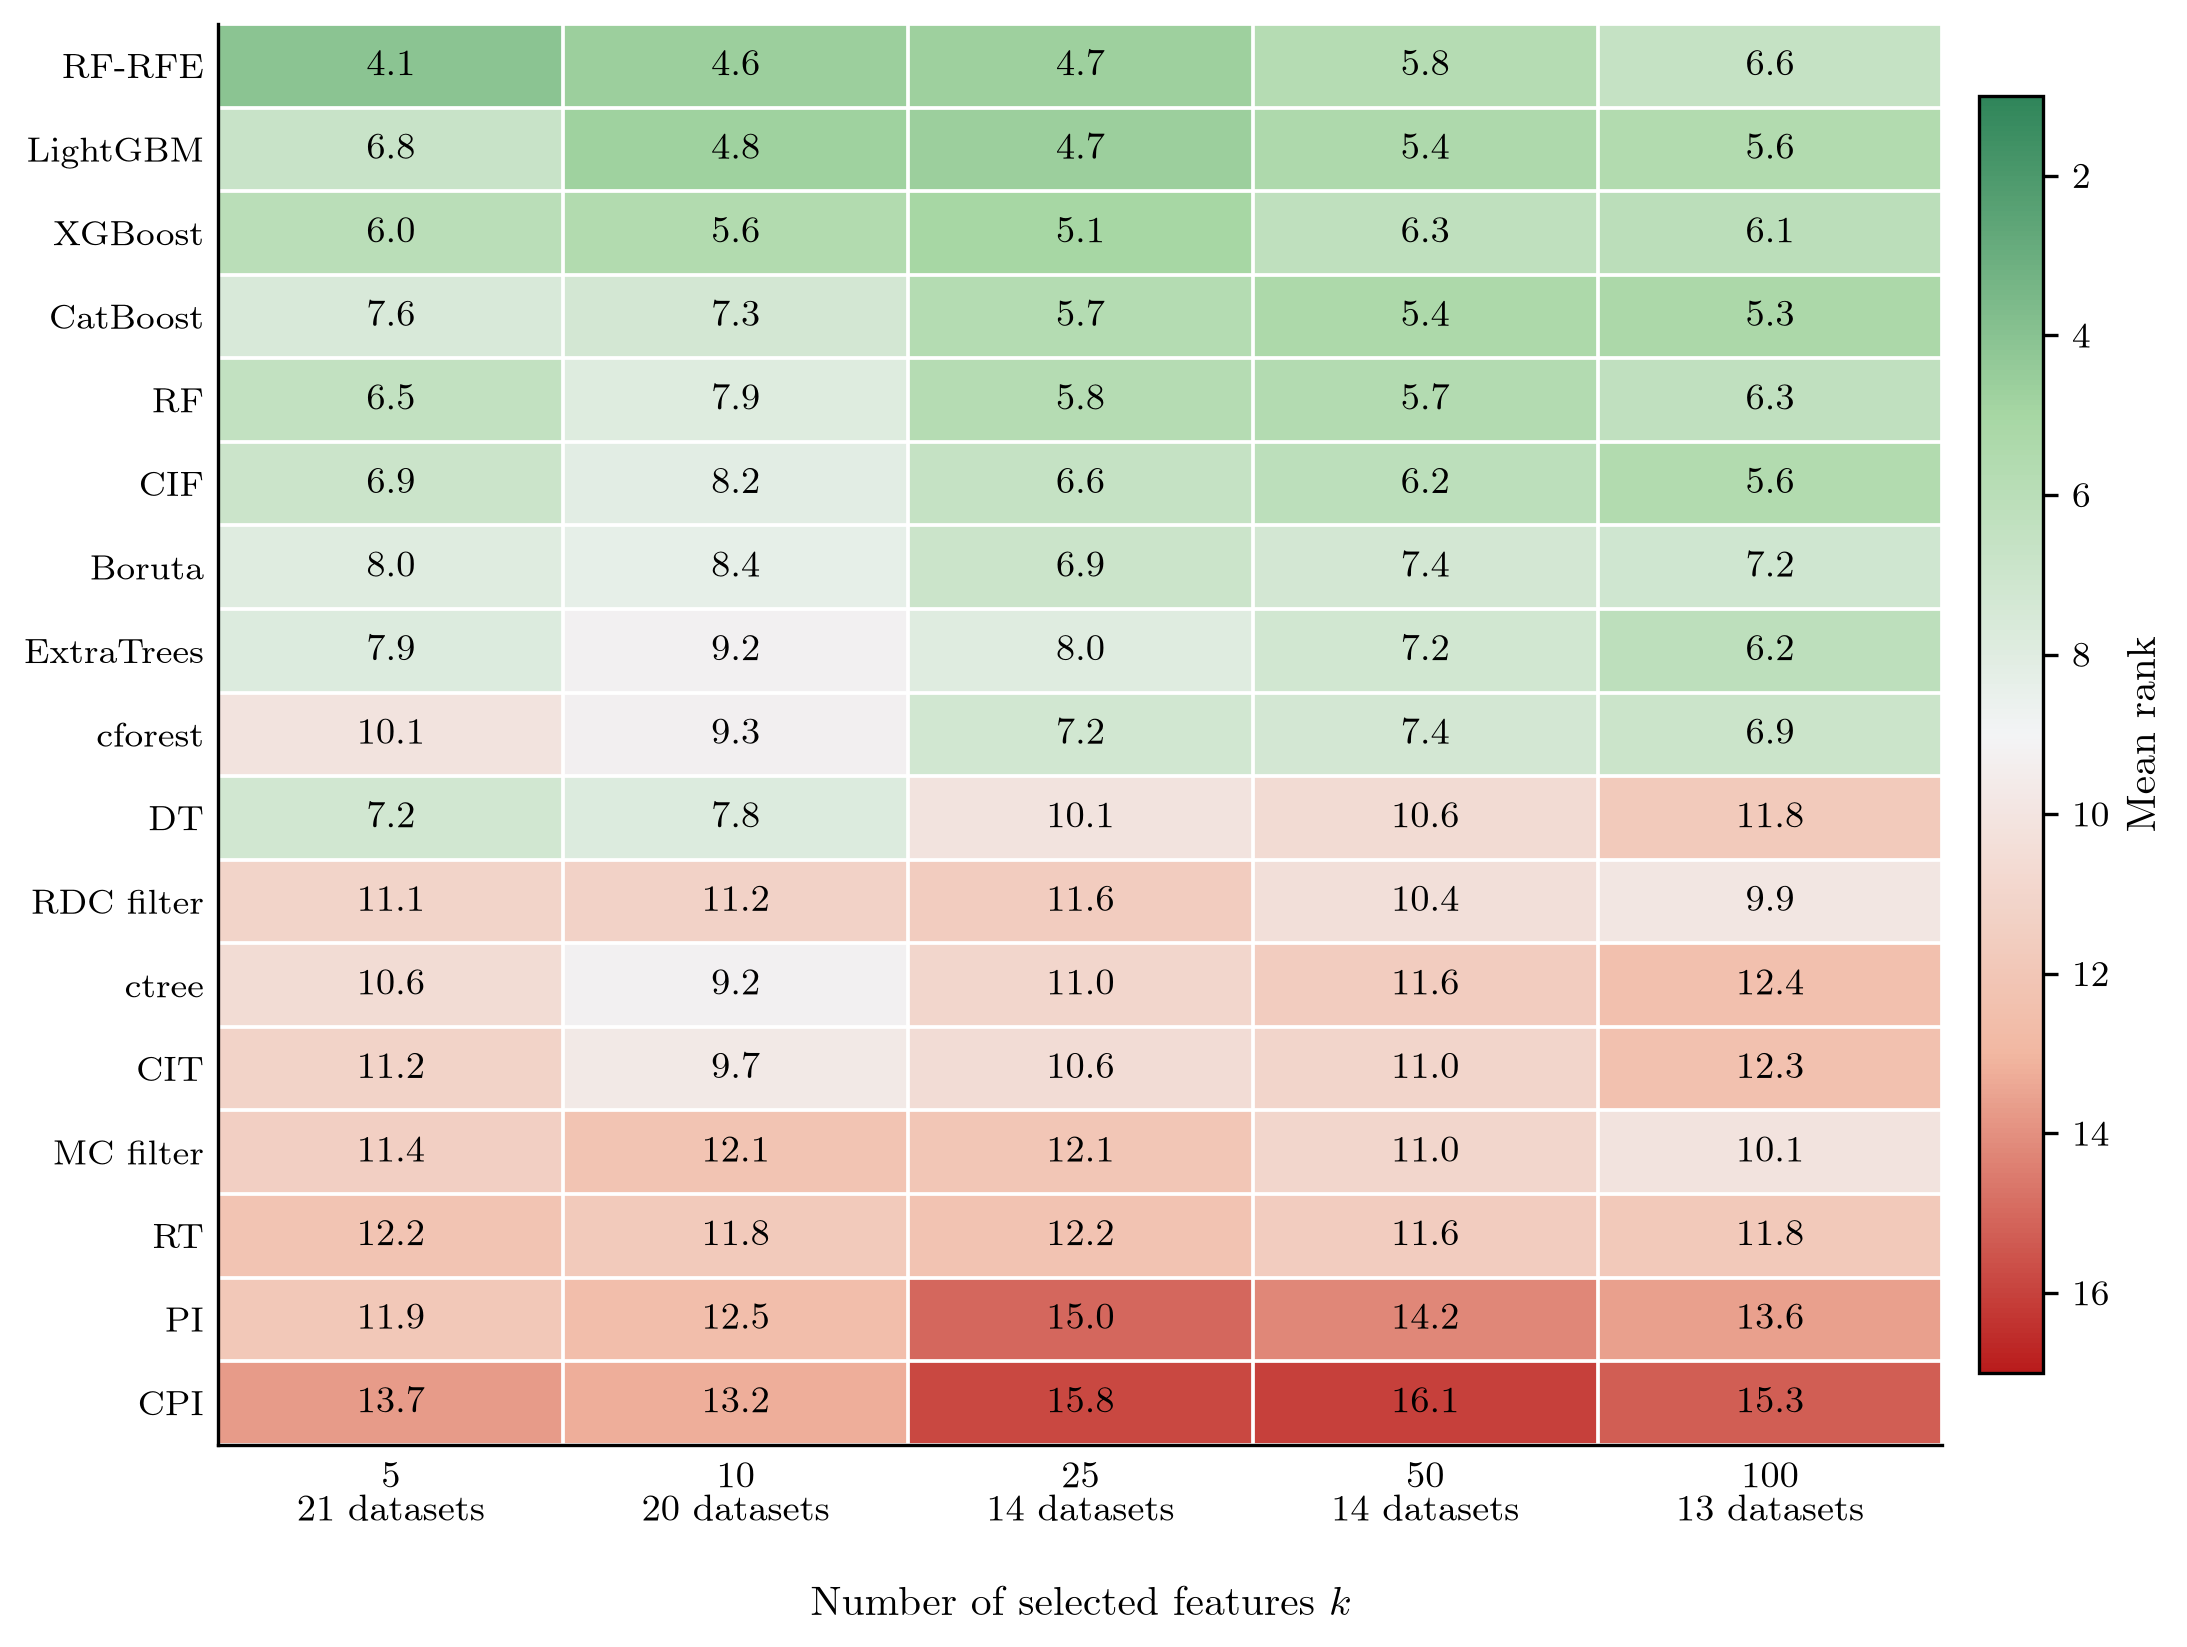
\includegraphics[width=0.86\linewidth]{figures/classification_k_trajectory.png}
  \caption{Classification mean rank by number of selected features. Rows show
  all 17 feature selection methods, averaged across downstream models at each
  value of $k$; lower ranks are better. The columns for $k=5,10,25,50,100$ use
  21, 20, 14, 14, and 13 datasets.}
  \label{fig:k-trajectory}
\end{figure}

\begin{figure}[!htbp]
  \centering
  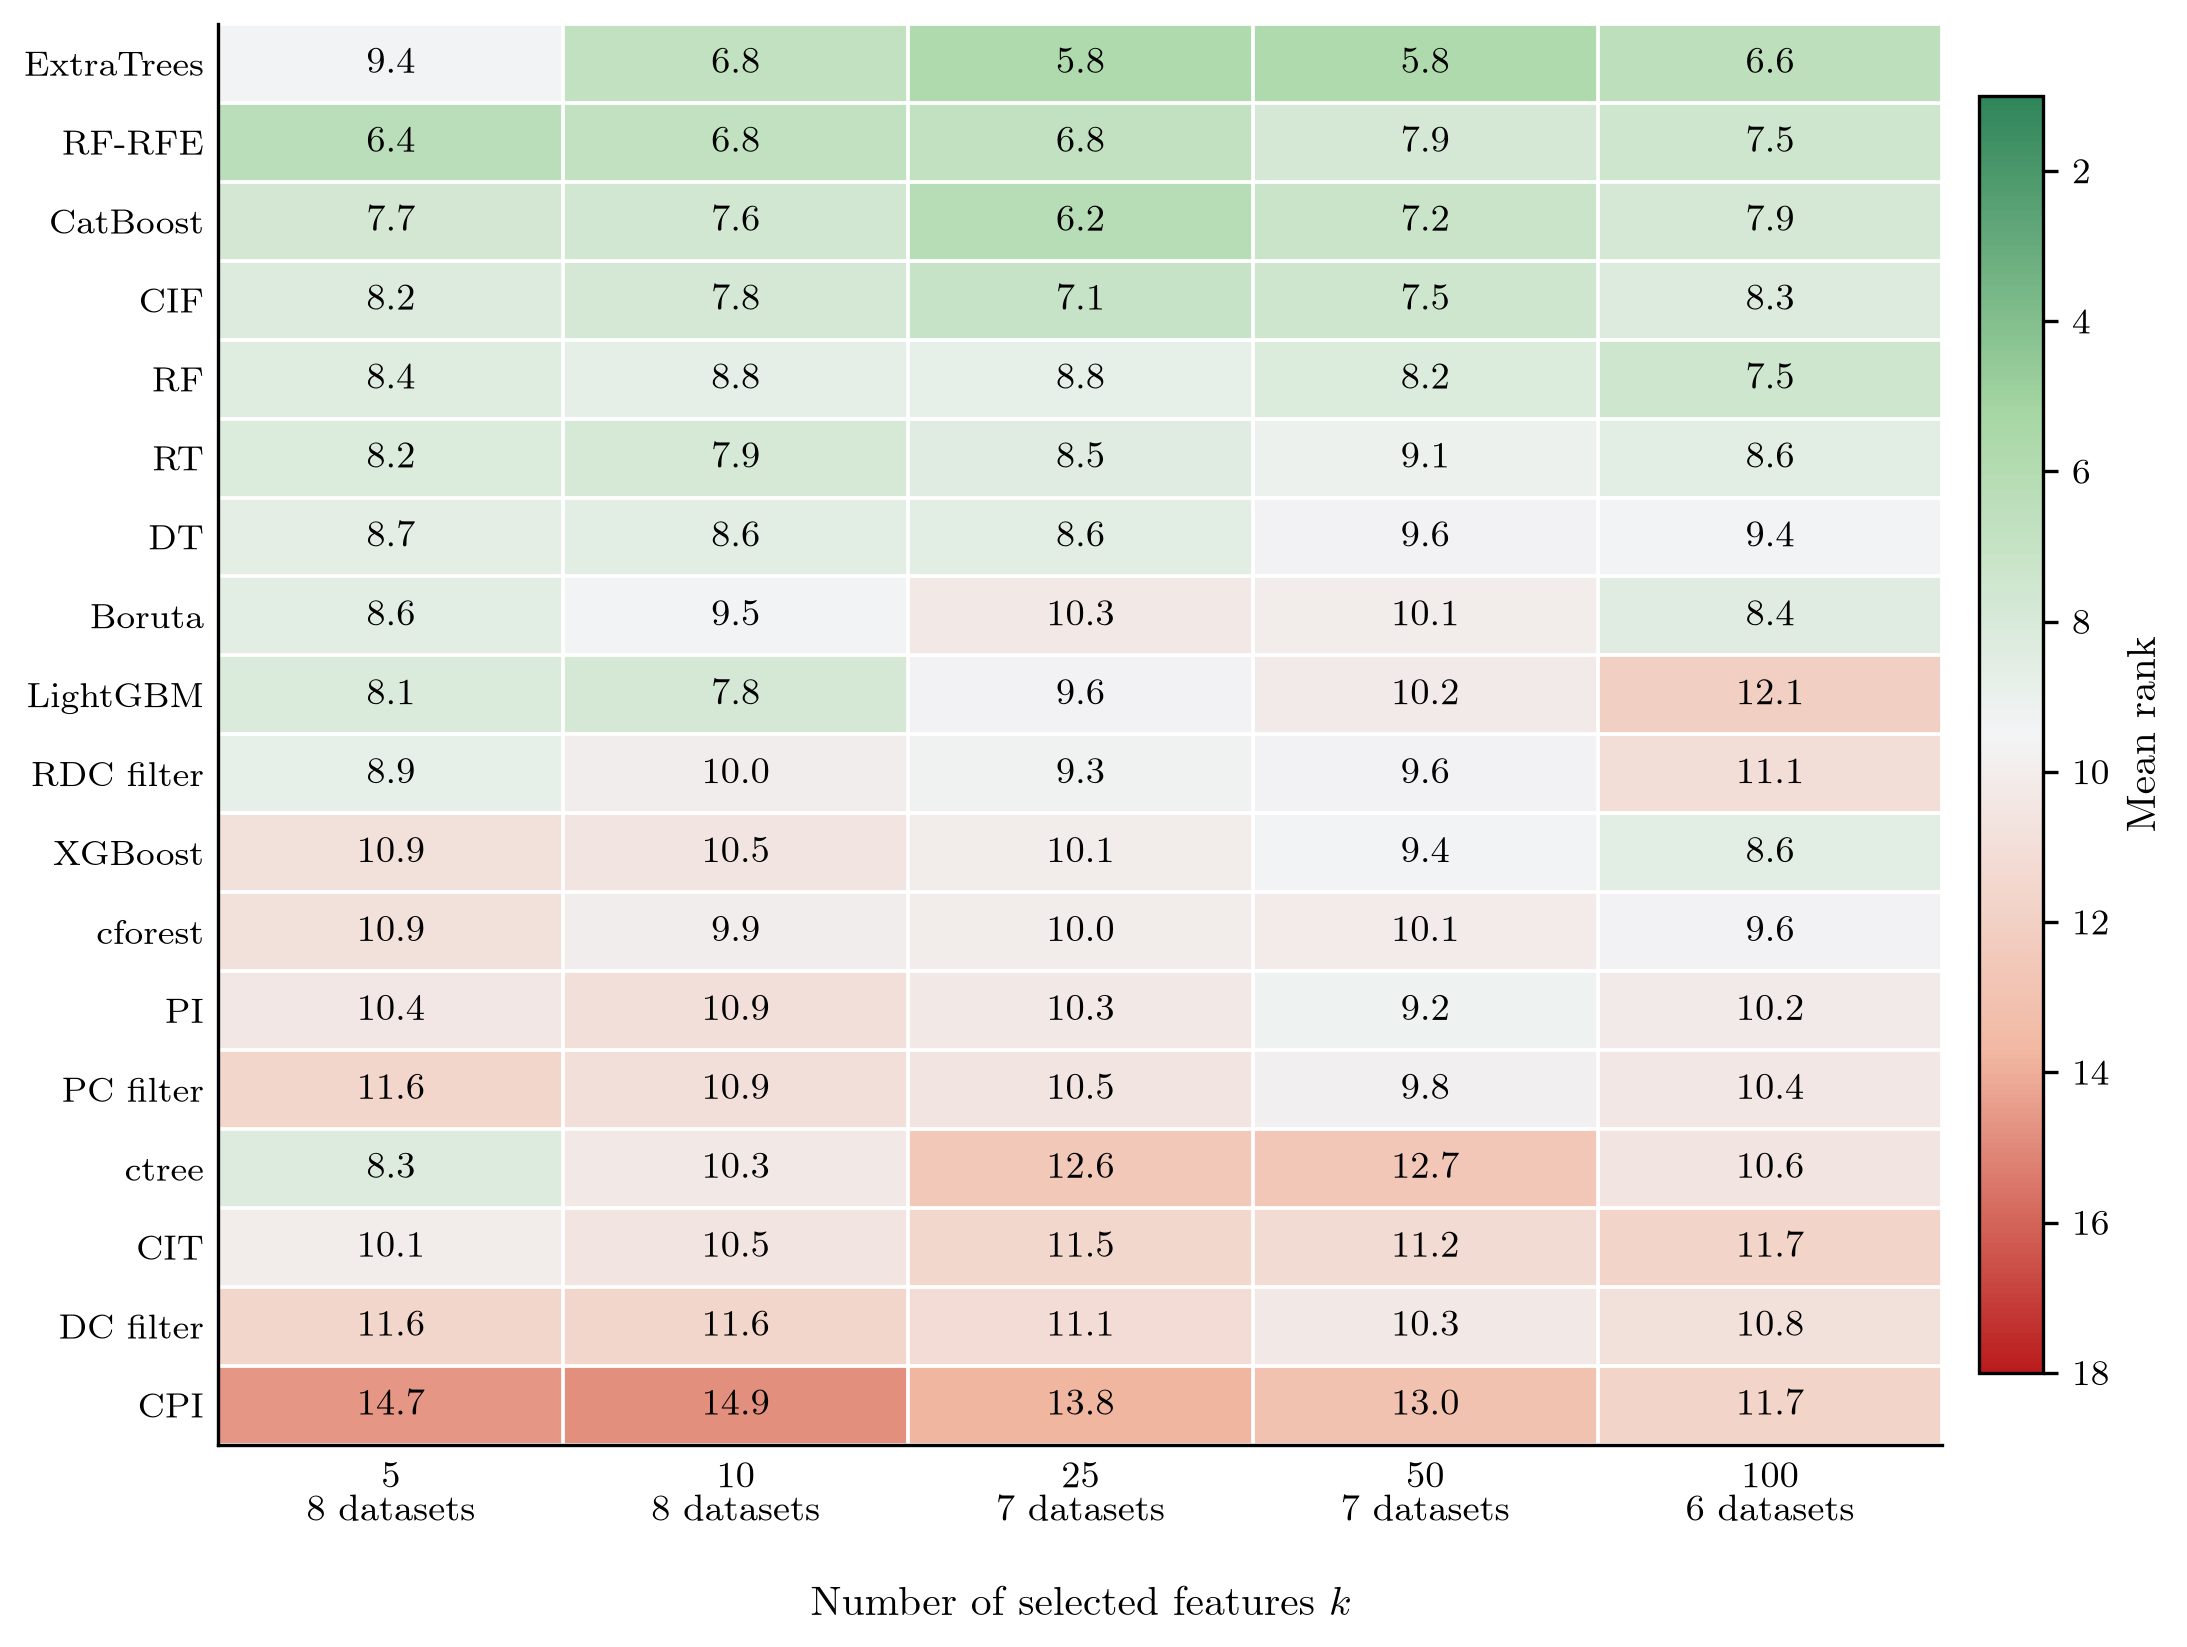
\includegraphics[width=0.86\linewidth]{figures/regression_k_trajectory.png}
  \caption{Regression mean rank by number of selected features. Rows show all
  18 feature selection methods, averaged across downstream models at each value
  of $k$; lower ranks are better. The columns for $k=5,10,25,50,100$ use 8, 8,
  7, 7, and 6 datasets.}
  \label{fig:regression-k-trajectory}
\end{figure}

\FloatBarrier
